\documentclass[a4paper,10pt, spanish]{article}

%%%%%%%%%% COMIENZO DEL PREAMBULO %%%%%%%%%%

%%%%%% DATOS INICIALES
%\author{...., Federico A. Ocampo}
%\title{Trabajo Pr'actico 1 Bases de Datos}

%%%% PAQUETES

%\usepackage{infostyle}  %%Se reemplaza por los siguientes.

\usepackage[top=3cm, bottom=3cm, left=3cm, right=3cm]{geometry}  % márgenes
\usepackage[utf8]{inputenc}                 % permite que los acentos del estilo áéíóú salgan joya
\usepackage[spanish, activeacute]{babel}    % idioma español, acentos fáciles y deletreo de palabras
\selectlanguage{spanish}
\usepackage{indentfirst}                    % permite indentar un parrafo a mano
\usepackage{wrapfig}                        % permite wrappear una figura
\usepackage{graphicx}                       % permite insertar gráficos
\usepackage{color}                          % permite el uso de colores en el documento
\usepackage{listings}                       % formatea código fuente
\usepackage{ulem}                           % Linea de puntos piola
% \usepackage[section]{algorithm}
% \usepackage{algpseudocode}                  % formatea pseudocod
\usepackage{caratula}                       % incluye caratula estándar
\usepackage[font=footnotesize,labelfont=normal]{caption} %modifica apariencia de los captions

%Extras de AMS para matematicas
% \usepackage{amsthm}     %ambiente para Teoremas
% \usepackage{amsmath}    %ambientes y comandos (ej: align, eqref)
% \usepackage{amsfonts}   %fuentes
% \usepackage{amssymb}    %Simbolos matematicos

% \ifpdf
% \usepackage[pdfcreator={Kile(r) bajo GNU/Linux},
            % pdfauthor={Grupo: 16},
            % pdftitle={TP MetNum},
            % pdfsubject={Trabajo Practico de Metodos Numericos},
            % pdfkeywords={Biseccion,Newton,Aritmetica Finita},
            % pdfstartview=FitH,            % Fits the width of the page to the window
            % bookmarksnumbered,            % los bookmarks numerados se ven mejor...
            % colorlinks,                   % links con bellos colores
            % linkcolor=blue]               % permite cambiar el color de los links
            % {hyperref}                    % Permite jugar con el PDF
% \fi

%%%%% FORMATO
\linespread{1.3}                          % interlineado equivalente al 1.5 líneas de Word...
\parskip=1.5ex                            % Un poco mas de espacio entre parrafos

\pagestyle{myheadings}              %encabezado personalizable con \markboth{}{}
\markboth{}{Bases de Datos - TP1}
\headsep = 30pt                     % separación entre encabezado y comienzo del párrafo

%define el lenguaje de prog a usar
\lstset{language=SQL}
\lstset{frame=single}

%%%%%% MACROS & COMANDOS
% macro 'todo' para To-Do's
\def\TODO#1{\textcolor{red}{#1}}
\newcommand{\real}{\hbox{\bf R}}
\newcommand{\entero}{\hbox{\bf Z}}

%inicializa el ambiente Teorema
% \newtheorem{theorem}{Teorema}[section]
% \newtheorem{propo}{Proposici\'on}[section]
% \newtheorem{definition}{Definici\'on}[section]

% Macro 'borde' para un texto con borde
\newsavebox{\fmbox}
\newenvironment{borde}[1]
{\begin{lrbox}{\fmbox}\begin{minipage}{#1}}
{\end{minipage}\end{lrbox}\fbox{\usebox{\fmbox}}\\[10pt]}

%%%%%%%%%% FIN DEL PREAMBULO %%%%%%%%%%

\begin{document}

\materia{Base De Datos}
\submateria{Trabajo Pr\'actico 1}
\titulo{Base de Datos del Torneo Sudamericano de Basket}
\integrante{Aronson, Alex}{443/08}{alexaronson@gmail.com}
\integrante{Nahabedian, Leandro }{250/08}{leanahabedian@hotmail.com}
\integrante{Ravasi, Nicol�s}{53/08}{nravasi@gmail.com}
\integrante{Ocampo, Federico}{599/02}{faocampo2004@yahoo.com.ar}
\maketitle

\section{Introducci\'on}
\label{sec:introduccion}

El proceso de dise\~no de las relaciones de una base de datos involucra muchos conceptos
tanto te\'oricos como pr\'acticos relacionados con los diferentes aspectos involucrados; 
no solamente es necesario definir que entidades entrar\'an en juego y las interrelaciones
entre si, sino tambi\'en tener en cuenta aspectos de redundancia de datos y de definici\'on de
los esquemas de forma tal que se aprovechen las interrelaciones existentes.

La creaci\'on de esquemas de bases de datos a nivel industrial solamente exige ciertos
 niveles de formalidad y de correctitud, pero en el aspecto te\'orico existen muchos estudios
que definen mejoras tanto para la reducci\'on de redundancia de datos y dependencias como para
la verificaci\'on de correctitud en la definici\'on de los esquemas y las interrelaciones.

% El presente trabajo presenta un desarrollo completo del dise�o de las entidades y esquemas
 % de una base de datos basada en un caso de uso ficticio pero con posibles aplicaciones en el mundo real.

\section{Diagrama Entidad-Relaci\'on (DER)}

\subsection{Diagrama}
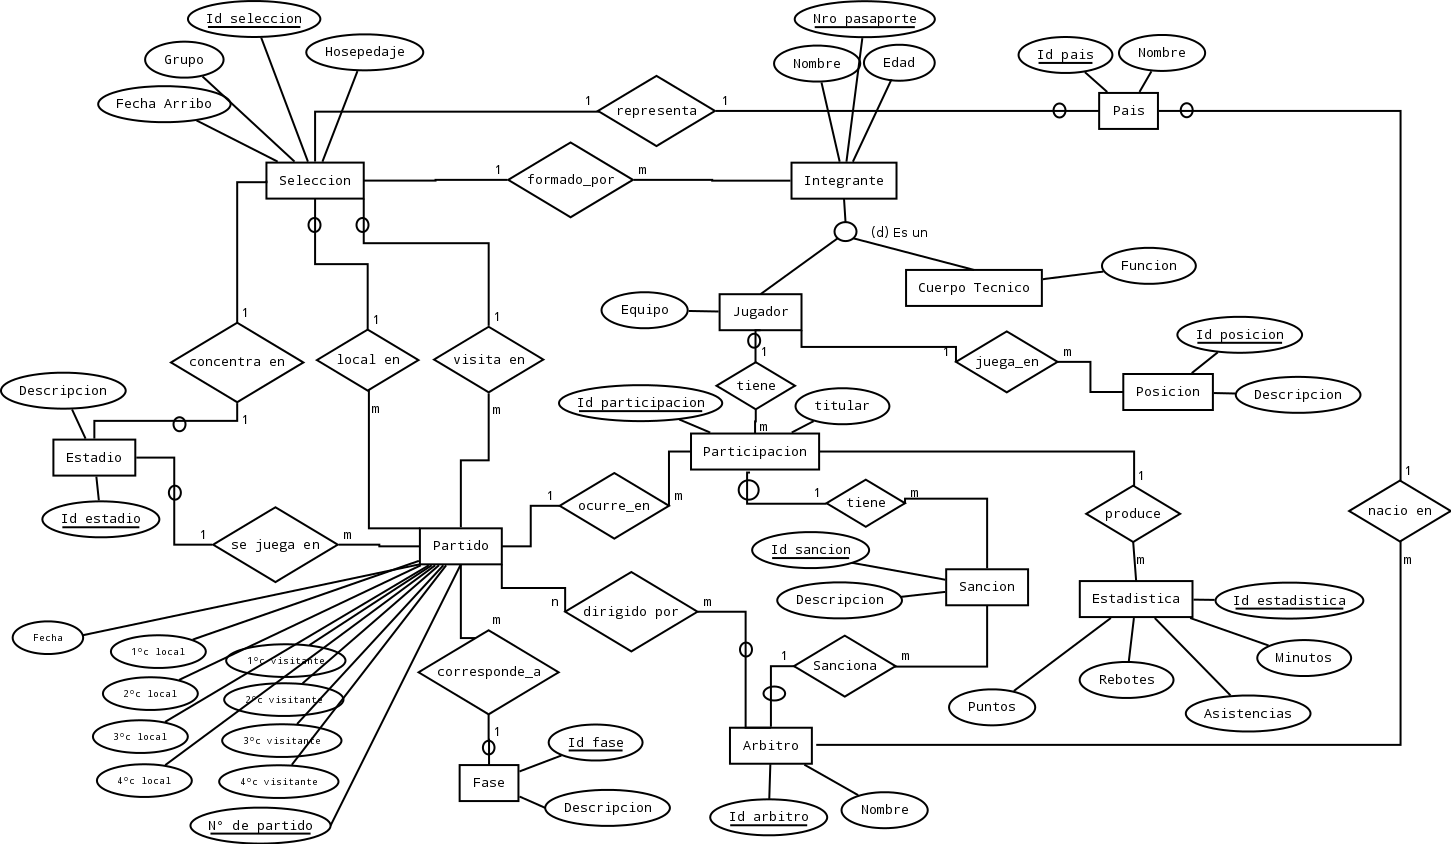
\includegraphics[scale=0.4, angle=90]{imgs/Der.png}


\newpage

\subsection{Decisiones de Dise\~no}


Para comenzar con el trabajo lo primero que hicimos fue tratar de identificar en el texto todo aquello que consderabamos que podia llegar a ser una entidad, para ellos seleccionamos del texto las palabras claves tales como, Jugador, Estadistica, Partido, Seleccion etc.
Luego detectamos que hab\'ia atributos tales, como pais y estadio que se usaban de manera repetidas, por lo que decidimos pasar a estas tambien en forma de Entidades.
Una vez con las entidades definidas nos propusimos llevar adelante la correcta diagramación de las interelaciones
Si bien no encontramos dificultades para poder relacionar las entidades, nos encontramos con una traba para poder relacionar al partido, con las estad\'isticas y con los jugadores
A primera instancia tratamos de trabajar con las estad\'isticas de forma que se generaban de manera agregada de la relaci\'on entre partido y jugador, sin embargo desistimos de esta opci\'on ya que no es posible que no exista estad\'istica alguna de un jugador que jugo un partido, por lo que no es necesario este tipo de relaci\'on.
Intentamos hacer una relaci\'on de grado 3 sin embargo tampoco creimos que era la manera correcta porque nos obligaba a inicializar una planilla de estadistica sobre todos los jugadores con valores en 0 y esto no es correcto, sino que las estad\'isticas se realizan sobre los jugadores que juegan. 
Finalmente decidimos implementar una entidad participaci\'on, encargada de administrar las estadisticas, si un jugador fue titular o no en ese partido y si tuvo o no sanciones.
A medida que ibamos diagramando nos encontramos con la necesidad de tomar decisiones para que el diagrama creado sea leído de manera correcta.

\begin{itemize}
\item Decidimos implementar la relaci\'on de partido con selecci\'on con dos relaciones distintas, la cual uno pertenece a una selecci\'on que hace el modo de Local y la otra de Visitante, es importante indicar que se debe restringir que esta selecci\'on no sea la misma, ya que esto es imposible en la realidad.
\item Por partido solo puede haber una cantidad de 12 jugadores correspondientes a cada equipo, es decir que si bien la relaci\'on es en base a $m$ este se limita a solamente 12
\item Se debe restringir que la cantidad de titulares de un partido sea igual a 5 tal como lo indica el trabajo para ello creamos un trigger en el cual si se intenta cargar un jugador como titular y ya se alcanzo la cantidad maxima, esa inserción falla.
\item Asumimos que la posici\'on de un jugador es propia del mismo e independientemente del partido, tal como es en la realidad de las estadisticas del basquet.
\item Permitimos que haya mas de un arbitro por partido, ya que entendemos que el enunciado asi lo pide refiriendose constantemente al terma arbitraje como plural
\item Si bien el partido tiene muchos \'arbitros, una sanci\'on puede ser aplicada por un solo \'arbitro.
\item Decidimos no colocar un campo de resultado final dentro de la tabla partido ya que este campo se puede deducir de la suma de los cuartos correspondientes a cada selecci\'on.
\item Si bien el trabajo solicita que se almacenen solo las estad\'isticas de los mejores jugadores, tambien pide como item emitir un reporte de las mismas sobre todos los que jugaron, por lo que no solo almacenamos informacion de los mejores sino que la haremos sobre todos los jugadores con partidos en su haber.
\end{itemize}



\section{Modelo Relacional}
\label{sec:mer}

\subsection{Esquemas de Relaciones}

En las siguientes secciones se formalizan las entidades y relaciones propuestas en el
\textbf{Diagrama Entidad-Relaci\'on} mediante el esquema de 
\textbf{Modelo Relacional}, definiendo claves candidatas, primarias y for\'aneas para cada una de ellas.
Por otro lado definiremos las restricciones que tiene nuestro esquema.

Seleccion(\underline{IdSeleccion}, Grupo, Hospedaje, Fecha Arribo, \dotuline{IdPais}, \dotuline{IdEstadio})\\
PK = CK = {IdSeleccion}\\
FK = {IdPais, IdEstadio}\\

Pais(\underline{IdPais}, Nombre)\\
PK = {IdPais}\\
CK = {IdPais, Nombre}\\

Integrante(\underline{NroPasaporte}, Nombre, Edad, EsUn, \dotuline{IdSeleccion})\\
PK  = CK = {NroPasaporte}\\
FK = {IdSeleccion}\\

Cuerpo Tecnico (\underline{\dotuline{NroPasaporte}}, Funcion)\\
PK = CK = FK = {NroPasaporte}\\

Jugador(\underline{\dotuline{NroPasaporte}}, Equipo, \dotuline{IdPosicion} )\\
PK = CK = {NroPasaporte}\\
FK = {NroPasaporte, IdPosicion}\\

Participacion(\underline{IdParticipacion}, EsTitular, \dotuline{NroPasaporte, NroDePartido})\\
PK=CK = {IdParticipacion}\\
FK= {NroPasaporte, NroDePartido}\\

Sancion(\underline{IdSancion}, Descripcion, \dotuline{IdParticipacion} ,\dotuline{IdArbitro})\\
PK=CK = {IdSancion}\\
FK= {IdParticipacion, IdArbitro}\\

Estadistica(\underline{IdEstadistica}, Minutos, Asistencias, Rebotes, Puntos, {\dotuline{IdParticipacion})\\
PK=CK = {IdEstadistica}\\
FK={IdParticipacion}\\

Arbitro(\underline{IdArbitro}, Nombre, \dotuline{IdPais})\\
PK=CK={IdArbitro}\\
FK={IdPais}\\

Partido(\underline{NroPartido}, 1CuartoLocal, 2CuartoLocal, 3CuartoLocal, 4CuartoLocal, 1CuartoVisitante, 2CuartoVisitante, 3CuartoVisitante, 4CuartoVisitante, Fecha, \dotuline{IdFase}, \dotuline{IdArbitro}, \dotuline{IdSeleccionLocal}, \dotuline{IdSeleccionVisitante, IdEstadio})\\
PK=CK= {NroPartido}\\
FK={IdFase, IdArbitro, IdSeleccionLocal, IdSeleccionVisitante, IdEstadio}\\

Fase(\underline{IdFase}, Descripcion)\\
PK=CK={IdFase}\\

Estadio(\underline{IdEstadio}, Descripcion)\\
PK=CK={IdEstadio}\\

Posicion(\underline{IdPosicion}, Descripcion)\\
PK=CK={IdPosicion}\\

DirigidoPor(\underline{\dotuline{nroPartido, idArbitro}})\\
PK = CK = {(nroPartido, idArbitro)}\\
FK = {nroPartido, idArbitro}\\



\section{Funcionalidades de la Base de Datos}
 
\subsection{Introducci\'on}

En este trabajo tuvimos que realizar stored procedures y triggers para poder indicar los paises que iutulizaron a todos sus jugadores como local, luego tuvimos que efectuar un listado de estadisticas indicando el promedio de las mismas para todos los jugadores que tuvieron participaci\'on, y finalmente nos encotramos con la necesidad de entregar una lista de \'arbitros permitidos para dirigir un partido creado.
Por otro lado insertamos restricciones necesarias para que un arbitro no pueda dirigir partidos que juega la selecci\'on de su pa\'is, y tambien para evitar una incorrecta carga de datos en el sistema. Esto lo hicimos a trav\'es de triggers que fallan si no cumplen con las condiciones.


\subsection{Stored Procedures}

\subsubsection{Procedure 1}

\begin{verbatim}
USE `TP1BD`;
DROP procedure IF EXISTS `Selecciones_Usaron_Todos_Jugs`;

DELIMITER $$
USE `TP1BD`$$
CREATE PROCEDURE `TP1BD`.`Selecciones_Usaron_Todos_Jugs` ()
BEGIN

select 
    p.nombre
from
    Seleccion s,
    Pais p
where
    s.idPais = p.idPais
        and not exists( select 
            i.idSeleccion
        from
            Jugador j, Integrante i
        where
            s.idSeleccion = i.idSeleccion
                and j.nroPasaporte = i.nroPasaporte
                and j.nroPasaporte not in (select distinct
                    p.nroPasaporte
                from
                    participacion p
                where
                    p.esTitular))
and exists (select * from Partido p  where p.idSeleccionLocal = s.idSeleccion or p.idSeleccionVisitante = s.idSeleccion);


END$$

DELIMITER ;
\end{verbatim}


\subsubsection{Estadistica Jugadores}

\begin{verbatim}
USE `tp1bd`;
DROP procedure IF EXISTS `Estadisticas_Jugadores`;

DELIMITER $$
USE `tp1bd`$$
CREATE PROCEDURE `tp1bd`.`Estadisticas_Jugadores` ()
BEGIN
select 
    Nombre,
    Partidos_Jugados,
    Minutos,
    Puntos,
    Rebotes,
    Asistencias,
    (Puntos / Partidos_Jugados) Ptos_por_partido,
    (Asistencias / Partidos_Jugados) Asistencias_por_partido,
    (Rebotes / Partidos_Jugados) Rebotes_por_partido
from
    (select 
        p.nroPasaporte,
            i.Nombre,
            sum(minutos) Minutos,
            sum(rebotes) Rebotes,
            sum(puntos) Puntos,
            sum(asistencias) Asistencias,
            count(1) Partidos_Jugados
    from
        integrante i, estadistica e, participacion p
    where
        p.idParticipacion = e.idParticipacion
            and i.nroPasaporte = p.nroPasaporte
    group by p.nroPasaporte , i.Nombre
    order by Partidos_Jugados) Total
order by partidos_jugados desc;
END$$

DELIMITER ;
\end{verbatim}

\subsubsection{Trigger Valida Arbritro}

\begin{verbatim}
-- Define un nuevo caracter delimitador en lugar del ';'
DELIMITER $$
CREATE
    TRIGGER `validarAsignacionArbitro` BEFORE INSERT
    ON `tp1bd`.`dirigidopor`
    
	FOR EACH ROW BEGIN
		DECLARE idPaisArbitro INT(11);
        DECLARE idPaisLocal INT(11);
		DECLARE idPaisVisita INT(11);

		-- Id del Pais del Arbitro
		SELECT a.idPais INTO @idPaisArbitro
		FROM arbitro a
		WHERE a.idArbitro = NEW.idArbitro;

		-- Ids de los paises de los equipos local y visit
		SELECT s1.idPais, s2.idPais
		INTO @idPaisLocal, @idPaisVisita
		FROM seleccion s1, seleccion s2, partido p
		WHERE
			p.nroPartido = NEW.nroPartido
			AND s1.idPais = p.idSeleccionLocal
			AND s2.idPais = p.idSeleccionVisitante;

        IF @idPaisArbitro = @idPaisLocal OR @idPaisArbitro = @idPaisVisita THEN
            -- Para invalidar la operacion, hacemos un INSERT de NULL invalido
            SET NEW.nroPartido = NULL;
        END IF;
    END;$$
DELIMITER ;
-- Se repone el caracter delimitar por defecto
\end{verbatim}

\subsubsection{Trigger Valida Paises Diferentes}

\begin{verbatim}
-- Define un nuevo caracter delimitador en lugar del ';'
DELIMITER $$
CREATE
    TRIGGER `validarPaisesDiferentes` BEFORE INSERT
    ON `tp1bd`.`Partido`
    
	FOR EACH ROW BEGIN

        IF NEW.idSeleccionLocal = NEW.idSeleccionVisitante THEN
            -- Para invalidar la operacion, hacemos un INSERT de NULL invalido
            SET NEW.nroPartido = NULL;
        END IF;
    END;$$
DELIMITER ;
-- Se repone el caracter delimitar por defecto
\end{verbatim}

\subsubsection{Trigger valida Participaciones}

\begin{verbatim}
 -- Define un nuevo caracter delimitador en lugar del ';'
DELIMITER $$
CREATE
    TRIGGER `validarParticipaciones` BEFORE INSERT
    ON `tp1bd`.`participacion`
    
	FOR EACH ROW BEGIN
		DECLARE cantTitulares INT(11);
		DECLARE cantJugadores INT(11);
		DECLARE idPaisJugador INT(11);

		SELECT j.idSeleccion INTO @idPaisJugador
               FROM integrante j
               WHERE j.nroPasaporte = NEW.nroPasaporte;

		SELECT count(1) Cantidad_Jugadores 
		INTO @cantJugadores
		FROM participacion p , integrante i 
		WHERE p.nroPasaporte = i.nroPasaporte and p.nroPartido = NEW.nroPartido and i.idSeleccion = @idPaisJugador
		GROUP BY idSeleccion, nroPartido;

		SELECT count(1) Cantidad_Jugadores 
		INTO @cantTitulares
		FROM participacion p , integrante i 
		WHERE p.nroPasaporte = i.nroPasaporte and p.nroPartido = NEW.nroPartido and i.idSeleccion = @idPaisJugador
				and esTitular 
		GROUP BY idSeleccion, nroPartido;

        IF @cantJugadores >= 12  or (@cantTitulares >=5 and new.esTitular) THEN
            -- Para invalidar la operacion, hacemos un INSERT de NULL invalido
            SET NEW.idParticipacion = NULL;
        END IF;
    END;$$
DELIMITER ;
-- Se repone el caracter delimitar por defecto
\end{verbatim}






\begin{thebibliography}{Databases}

\bibitem[RG97]{Ramakrishnan1997}
Raghu Ramakrishnan and Johannes Gehrke.
\newblock {\em Database Management Systems}.
\newblock McGrawHill, second edition edition, 1997.

\bibitem[DB07]{Modelizacion}
C{\'a}tedra Bases de Datos.
\newblock Apunte de modelizaci{\'o}n.
\newblock Apunte de Modelizaci{\'o}n, Marzo 2009.

\bibitem[TYF86]{Teory1986}
Toby~J. Teory, Dongqing Yang, and James~P. Fry.
\newblock A logical design metodology for relational databases using the
  extended entity-relationship model.
\newblock {\em Computing Surveys}, 18(2), jun 1986.

\bibitem[MY09]{MySQL Web Site}
\newblock MySQL Official Documentation.
\newblock http://dev.mysql.com.

\end{thebibliography}


% \appendix
% \include{ApendiceA} %Enunciado 
\end{document}
